% Unofficial Umich Poster template.
% A fork of the MSU template https://www.overleaf.com/latex/templates/an-unofficial-poster-template-for-michigan-state-university/wnymbgpxnnwd
% which is a fork of https://www.overleaf.com/latex/templates/an-unofficial-poster-template-for-new-york-university/krgqtqmzdqhg
% which is a fork of https://github.com/anishathalye/gemini
% also refer to https://github.com/k4rtik/uchicago-poster



\documentclass[final]{beamer}

% ====================
% Packages
% ====================

\usepackage[T1]{fontenc}
\usepackage[utf8]{luainputenc}
\usepackage{lmodern}
\usepackage[size=custom, width=122,height=91, scale=1.2]{beamerposter}
\usetheme{gemini}
\usecolortheme{msu}
\usepackage{graphicx}
\usepackage{booktabs}
\usepackage{tikz}
\usepackage{pgfplots}
\pgfplotsset{compat=1.14}
\usepackage{anyfontsize}

% ====================
% Lengths
% ====================

% If you have N columns, choose \sepwidth and \colwidth such that
% (N+1)*\sepwidth + N*\colwidth = \paperwidth
\newlength{\sepwidth}
\newlength{\colwidth}
\setlength{\sepwidth}{0.025\paperwidth}
\setlength{\colwidth}{0.3\paperwidth}

\newcommand{\separatorcolumn}{\begin{column}{\sepwidth}\end{column}}

% ====================
% Title
% ====================

\title{Modelling deleterious load accumulation in locally adaptive inversions}

\author{Alex Pinch and Gregory Owens, PhD.}

\institute[shortinst]{Department of Biology, University of Victoria}

% ====================
% Footer (optional)
% ====================

\footercontent{
 EVO-WIBO 2023, Poster 47 \hfill
 }
% (can be left out to remove footer)

% ====================
% Logo (optional)
% ====================

% use this to include logos on the left and/or right side of the header:
% Left: institution
 \logoright{
\includegraphics[height=7cm]{images/logo.png}}
% Right: funding agencies and other affilations 
%\logoright{\includegraphics[height=7cm]{logos/NSF.eps}}
% ====================
% Body
% ====================

\begin{document}

\begin{frame}[t]
\begin{columns}[t]
\separatorcolumn

\begin{column}{\colwidth}

\begin{alertblock}{Summary}
We built a forwards-time population model in SLiM to see if a locally adaptive inversion accumulated less deleterious load than in a traditional underdominant scenario. To do this, we tracked deleterious mutation accumulation across these two scenarios. We would expect an \textbf{overdominant scenario} to show reduced recombination and thus \textbf{higher deleterious load}, while a \textbf{locally adaptive scenario} to have increased recombination and therefore \textbf{less deleterious load}. Generating models for these scenarios may offer valuable insights on why inversions do not frequently lead to detrimental phenotypes, compared to other large alterations in chromosome structure.
\end{alertblock}

  \begin{block}{Chromosomal inversions block recombination}

    When part of a chromosome becomes inverted, harmful mutations may not be purged due to disrupted recombination during meiosis. This causes the inversion to be inherited as a single block, trapping the genes within it. Over generations, the lost purging ability results in a build-up of harmful mutations, but the inversion may still persist if the genes trapped in the inversion are favourable.

    \begin{figure}
      \centering
    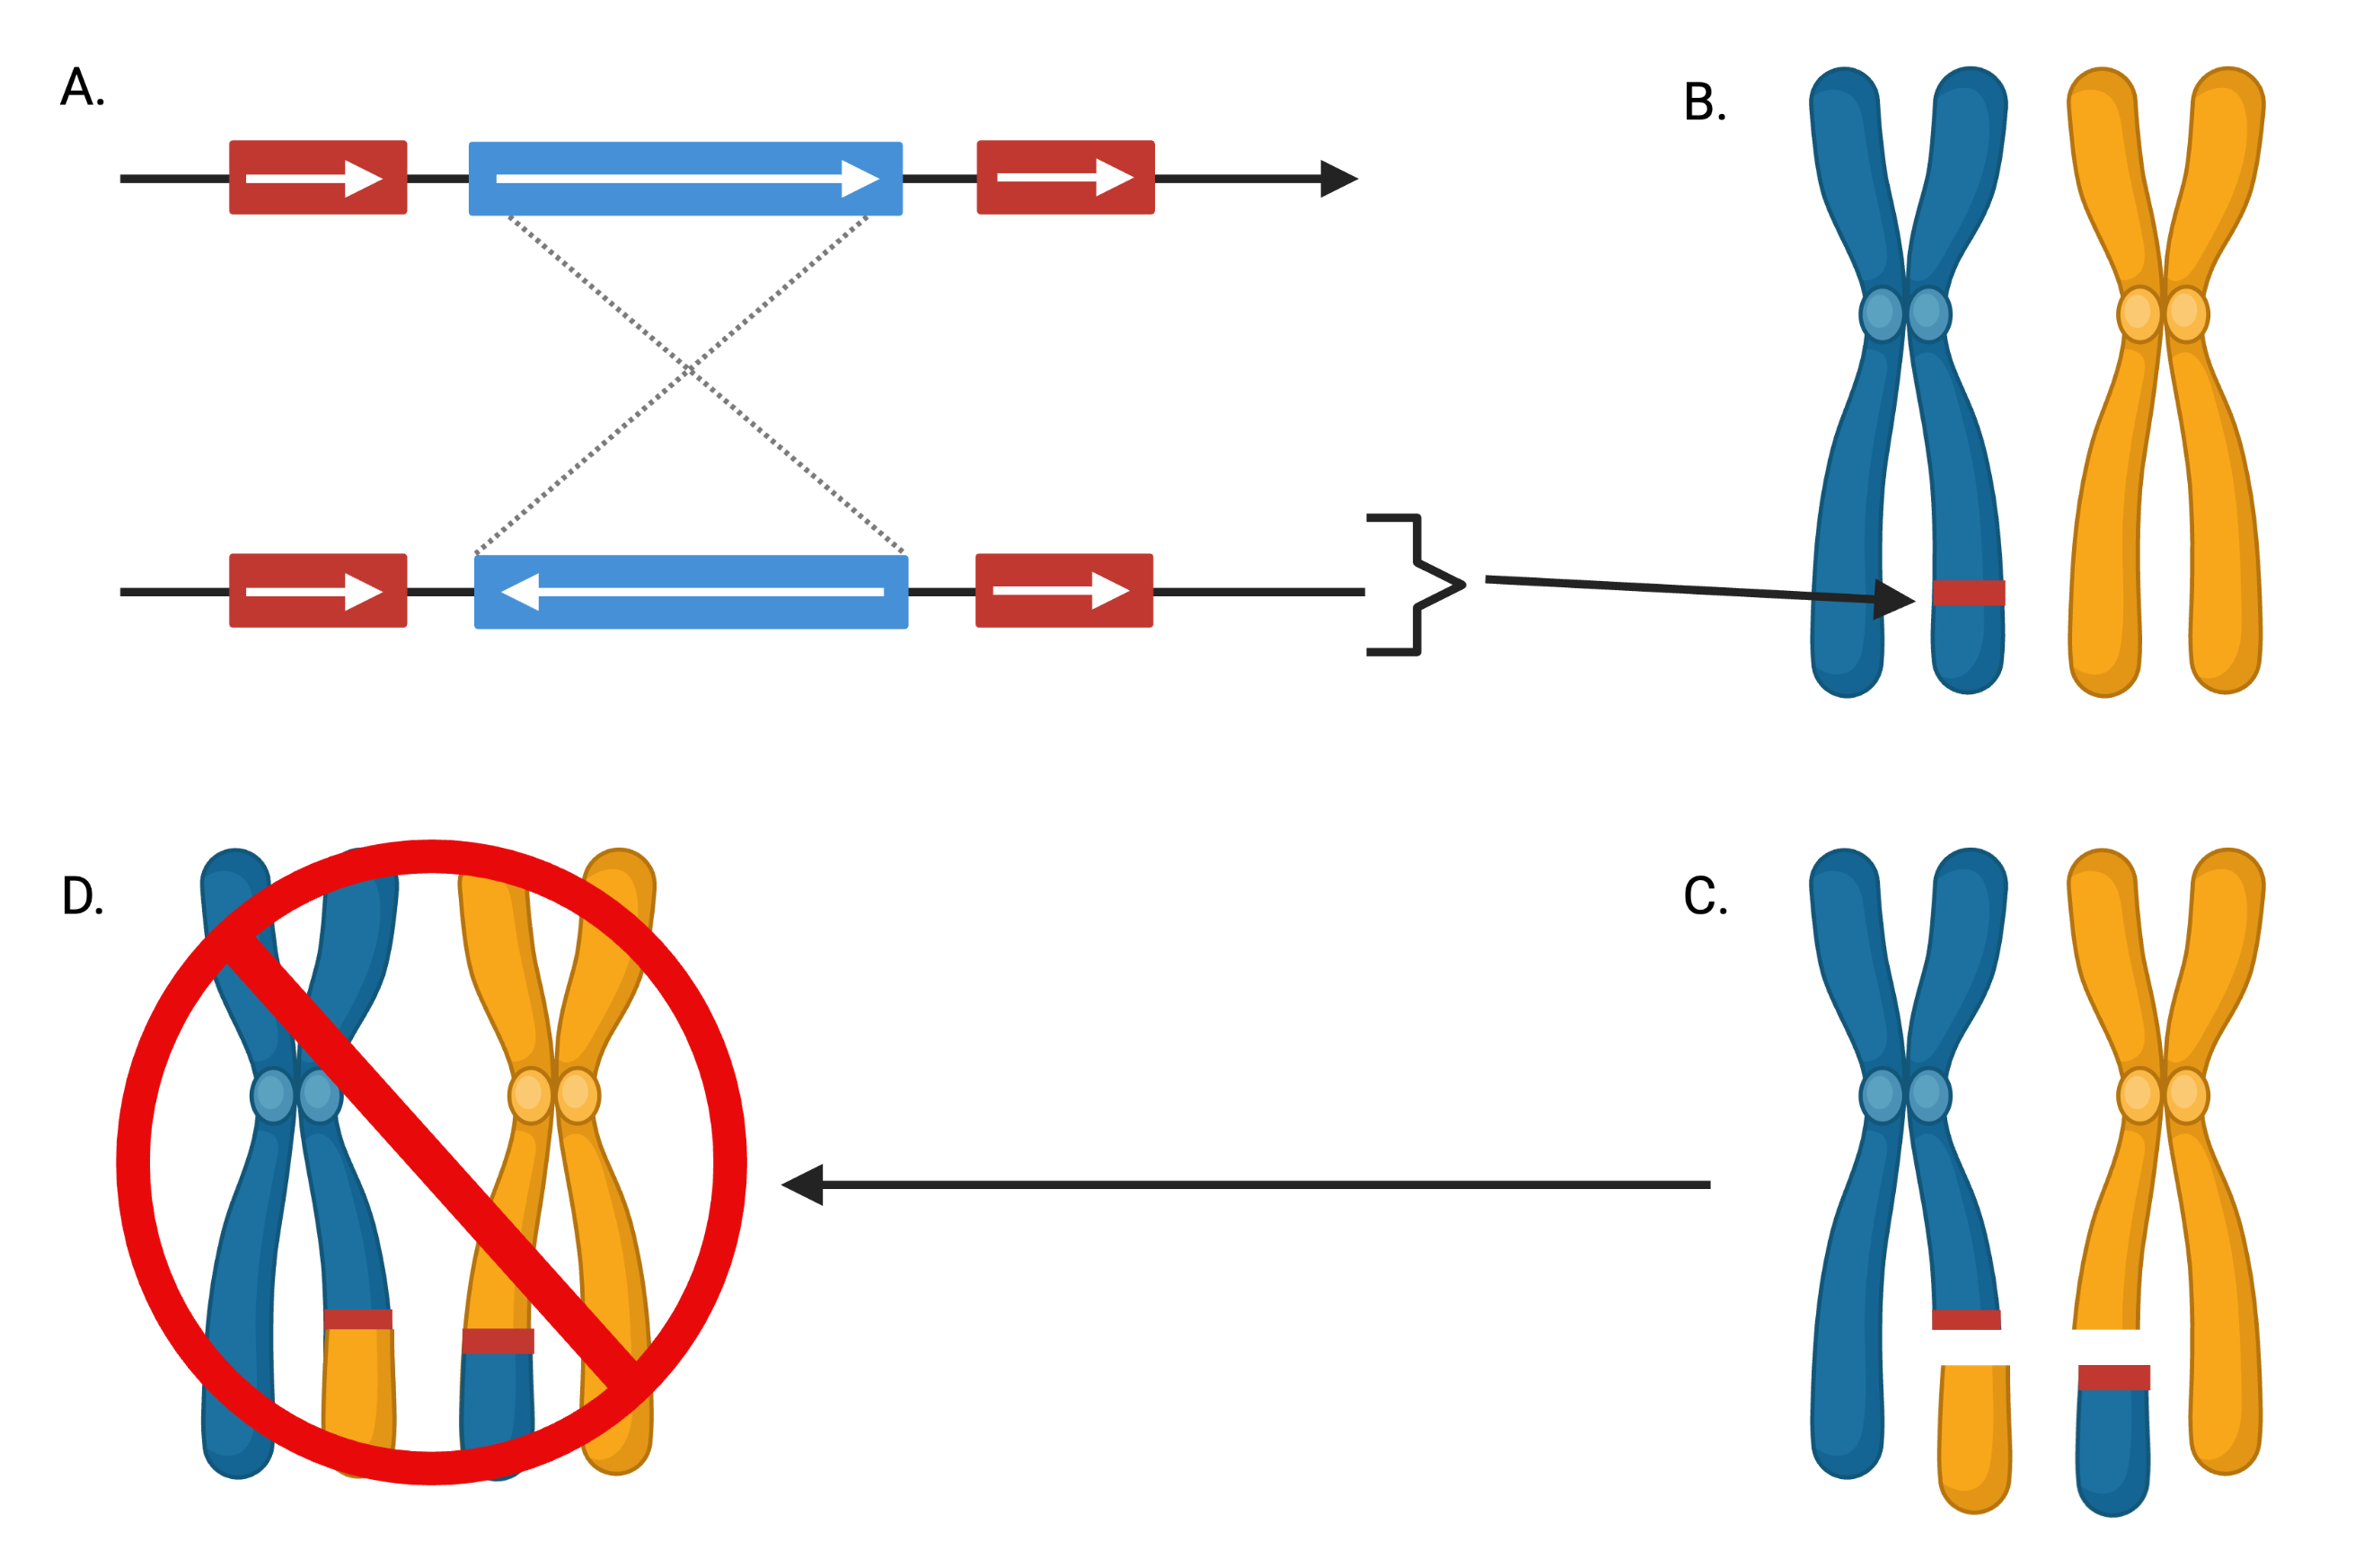
\includegraphics[width=0.6\textwidth]{images/chromosome.png}
    \caption{Meiosis between inverted and non-inverted chromosomes results in a malformed phenotype. Thus, recombination is prevented in individuals heterozygous for an inversion.}
    \end{figure}

    Two scenarios where an inversion may persist is in the case that it is overdominant or locally adaptive. If the genes trapped in the inversion are beneficial it will be favourable to be a heterozygote and lock those genes in. If the benefit of the inversion is dependent on the environment, as in the locally adaptive scenario, the homozygote will be favoured and the ability to purge harmful mutations may be rescued.

  \end{block}

  \begin{exampleblock}{Our model}

    Using SLiM, we built a model to simulate the rise of an inversion across a grid of populations. Mutations of varying fitness effects were allowed to accumulate over a 50k generation burn-in, after which a marker signifying the inversion was placed. This model was then amended for two scenarios:

    \begin{itemize}
      \item \textbf{A locally adaptive scenario}: Across a grid of populations, the fitness benefit of the inversion forms a gradient, in which the top left populations gains a 10\% fitness increase and the bottom right populations experience a 10\% decrease in fitness.
      \item \textbf{An overdominant scenario}: Across a grid of populations, the heterozygote confers a strict fitness benefit of 10\%.
    \end{itemize}

    Deleterious mutation frequency and fitness effects were pulled from a gamma-distribution and were always recessive. Each scenario was run 10,000 times, each run ended after 100,000 generations. Runs where the inversion died out were excluded.
    
  \end{exampleblock}

\end{column}

\separatorcolumn

\begin{column}{\colwidth}

    \begin{block}{A locally adaptive scenario}

        \begin{figure}
          \begin{minipage}[c]{0.3\textwidth}
            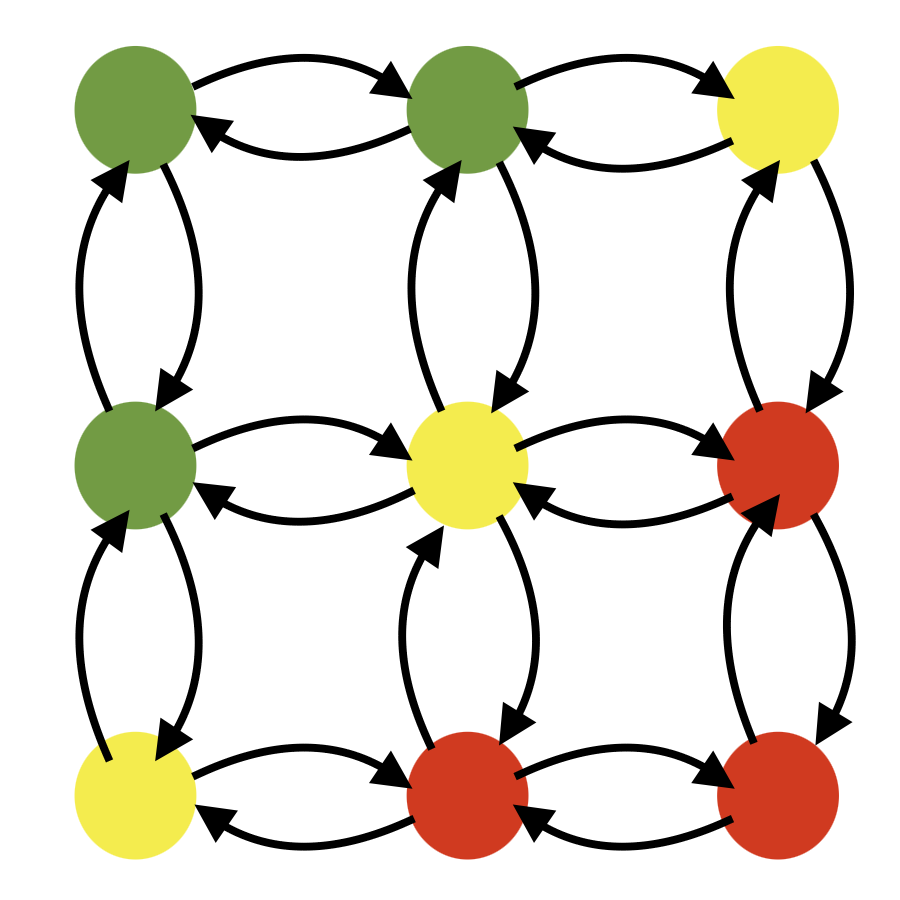
\includegraphics[width=0.9\textwidth]{images/la_populations.png}
          \end{minipage}\hfill
          \begin{minipage}[c]{0.67\textwidth}
            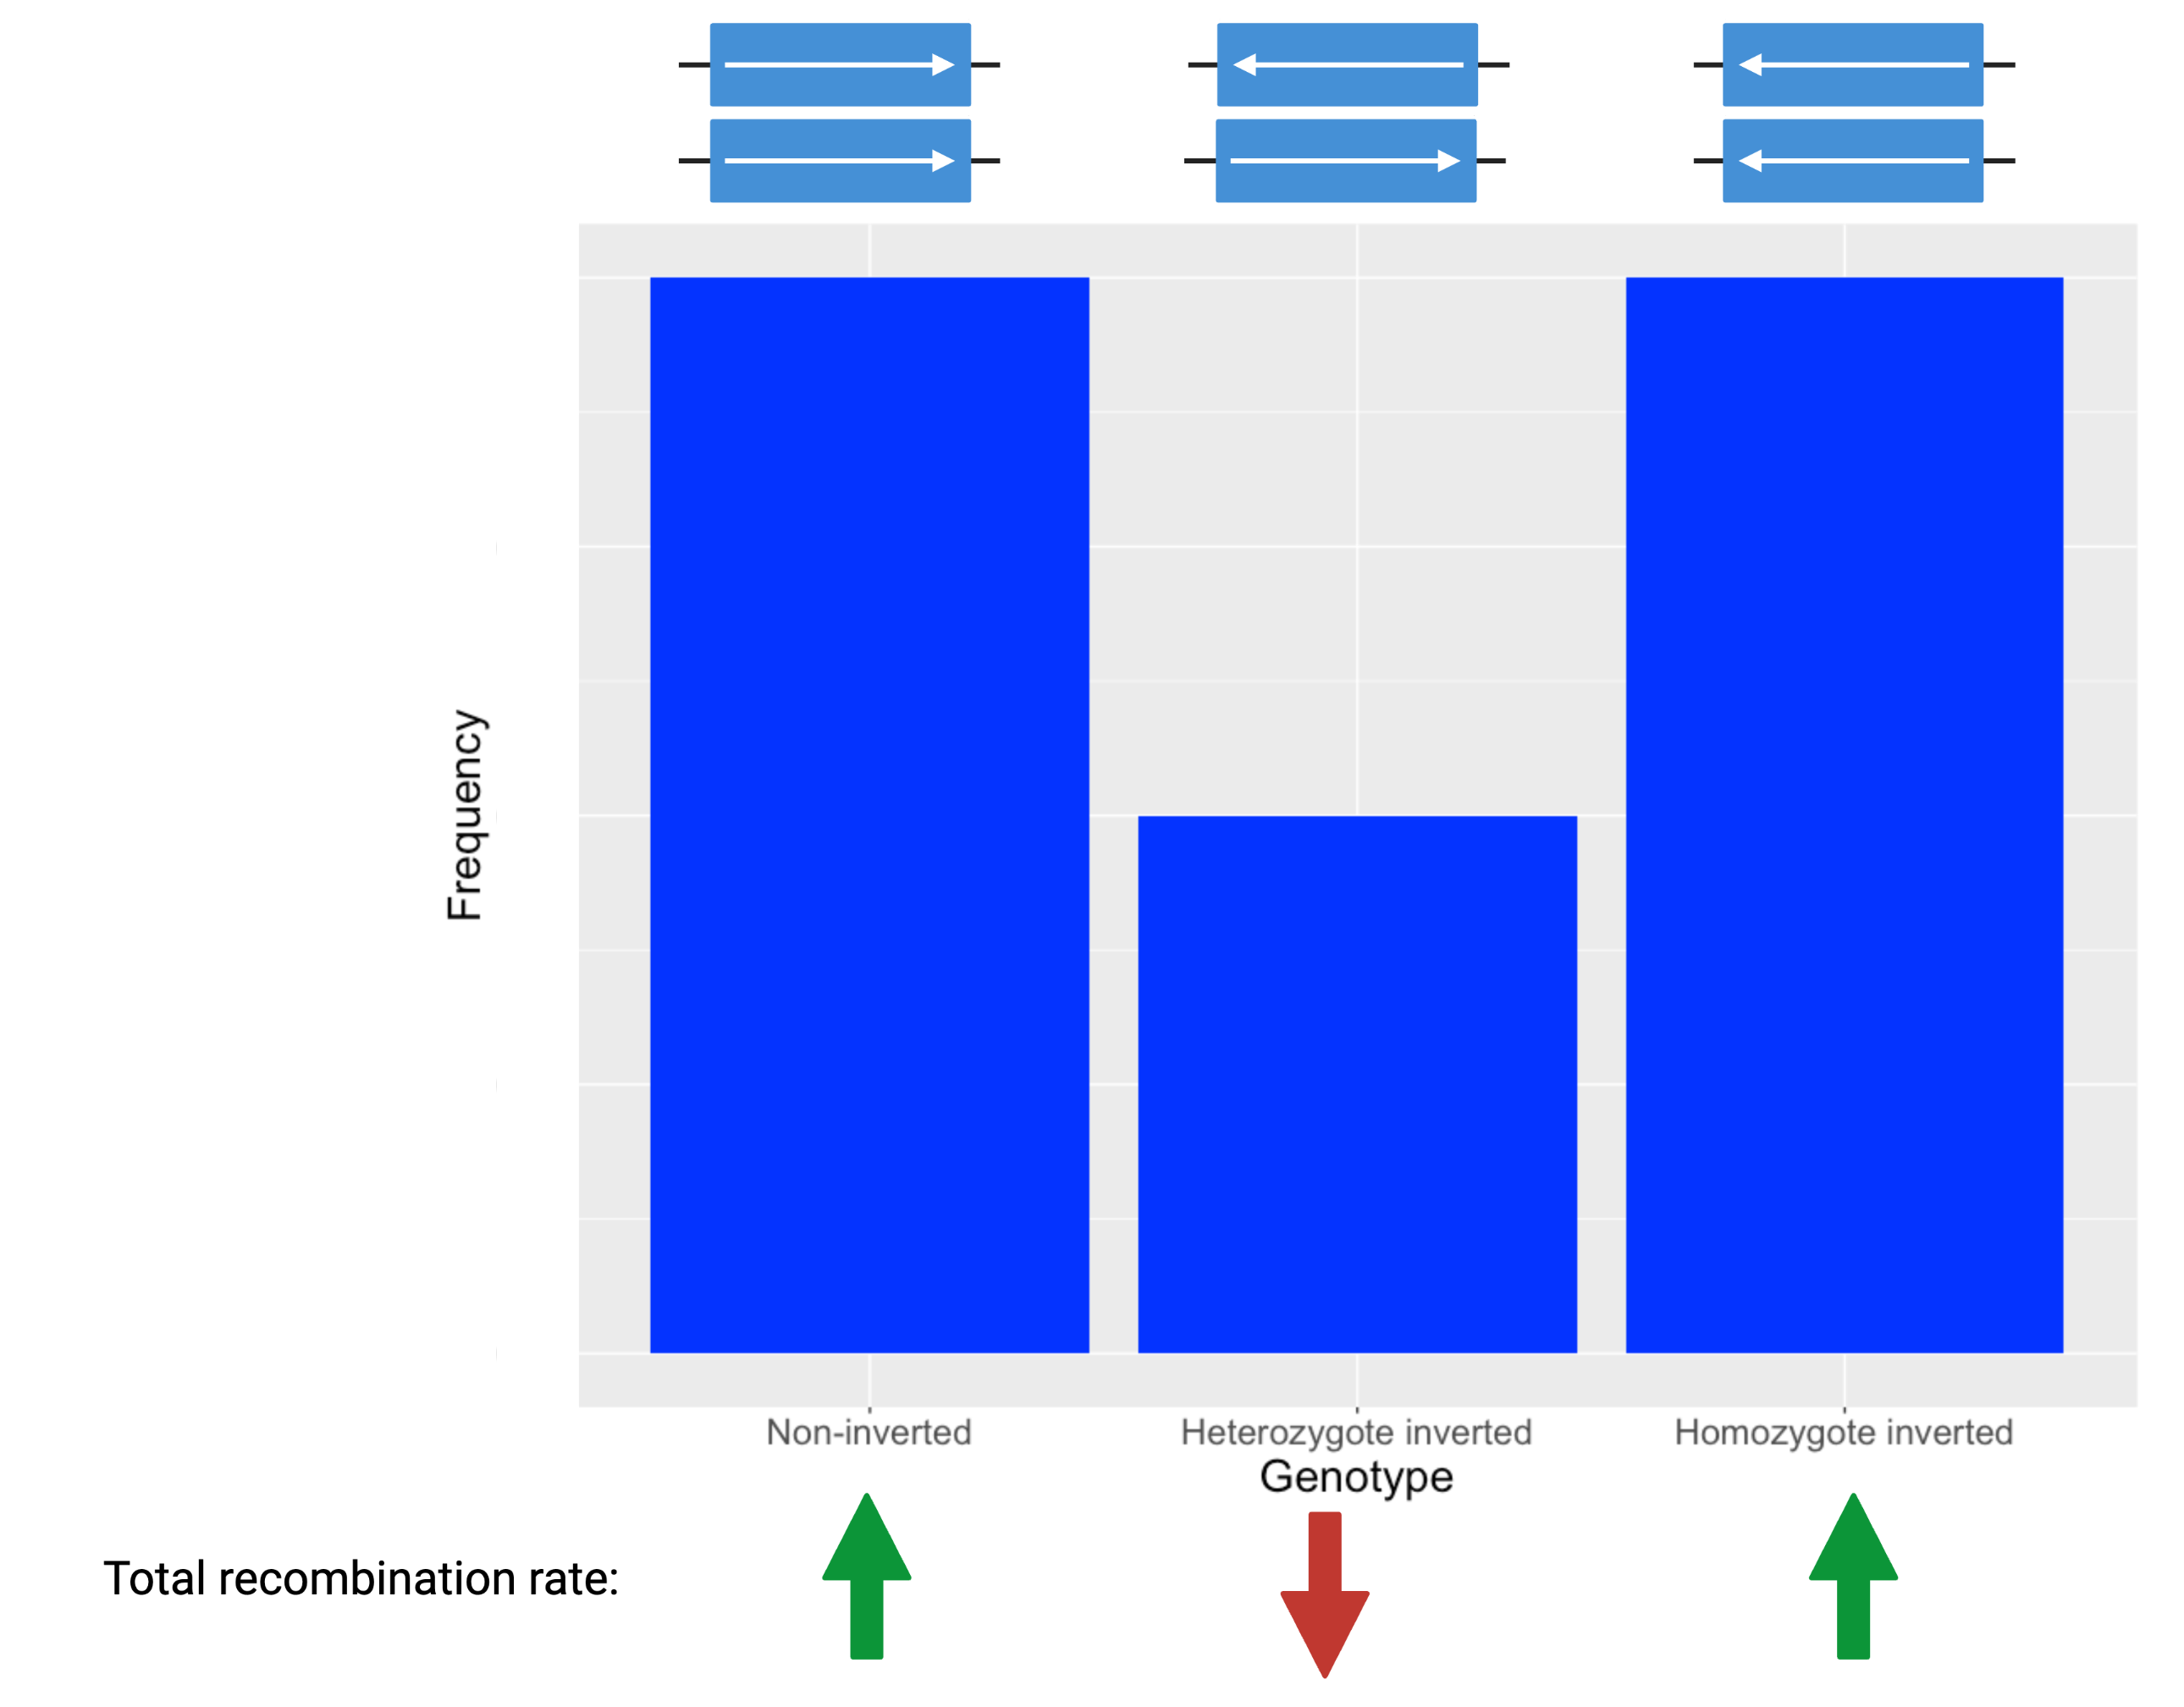
\includegraphics[width=0.9\textwidth]{figures/la_theory.png}
          \end{minipage}\hfill
          \caption{
            In the locally adaptive model, individuals with the inversion have higher fitness in the upper-left populations, but lower fitness in the lower-right populations, with no effect on the middle populations. As the number of homozygotes rise, recombination rate will increase and deleterious mutations will be purged.
            }
        \end{figure}
        
        In the locally adaptive scenario, heterozygotes are at a disadvantage as they gain half the benefit a homozygote would. In this case, the homozygote is favoured and should rise to higher frequency than the heterozygote. With less heterozygotes, the total recombination occurring in the population is increased. This mechanism may rescue the population from deleterious build-up.
    
        \begin{figure}
        \centering
                        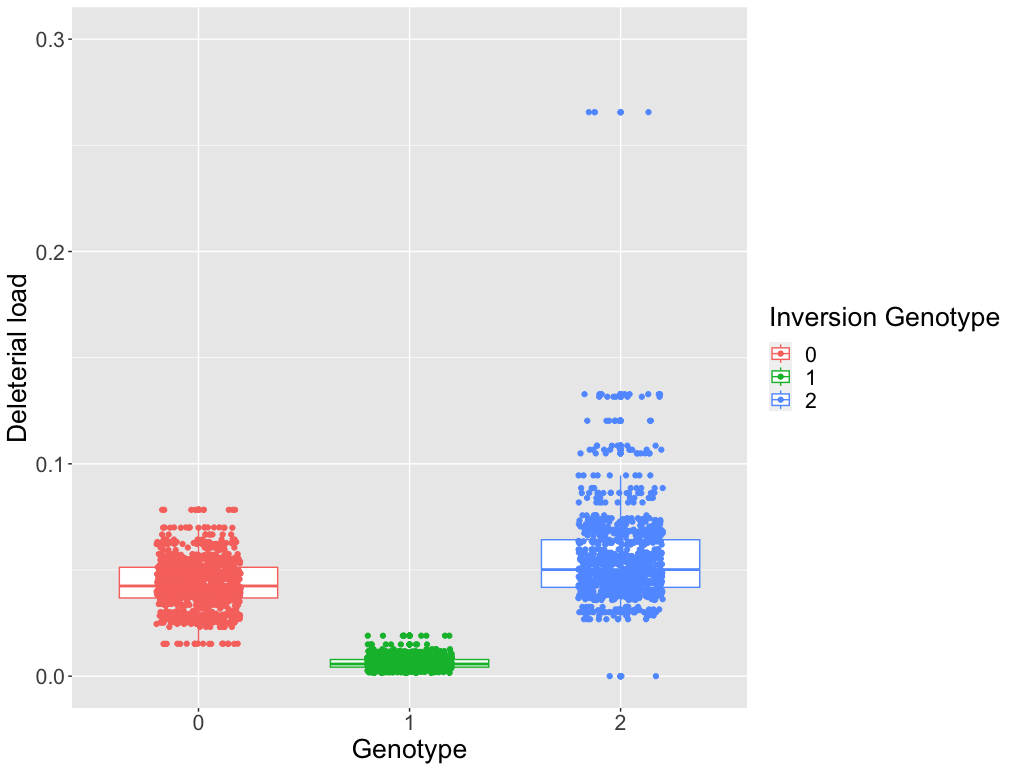
\includegraphics[width=0.5\textwidth]{figures/la_load_100kgen.png}
        \caption{A modelled locally adaptive inversion showed little deleterious load accumulation after 100,000 generations. After the fitness modifiers (+10\%/-10\%) were removed, deleterious load was calculated as 1 - fitness. }
        \end{figure}

    \end{block}
    \begin{exampleblock}{Tentative locally adaptive results}

        In the locally adaptive scenario, deleterious load accumulated \textbf{most in the homozygote} and \textbf{least in the heterozygote}. Recombination suppression in heterozygotes, as well as their lower sample size, may explain the reduced load in comparison to the homozygotes. Non-inverted individuals may have shown more accumulation than heterozygotes due to genetic drift: losing beneficial mutations in favour of the deleterious mutations increasingly prevalent across the populations. However, this still doesn't explain \textbf{why heterozygotes show almost no deleterious load}, and drift can't be acting on the non-inverted individuals alone. If genetic drift is causing the non-inverted load increase, how are heterozygotes not affected as well? Answers to these questions likely lie in the parameters of the model, such as the number generations run, or the frequency of the deleterious mutations at the end of the burn-in.

    \end{exampleblock}
    
\end{column}

\separatorcolumn

\begin{column}{\colwidth}

  \begin{block}{An overdominant scenario}

    \begin{figure}
          \begin{minipage}[c]{0.3\textwidth}
            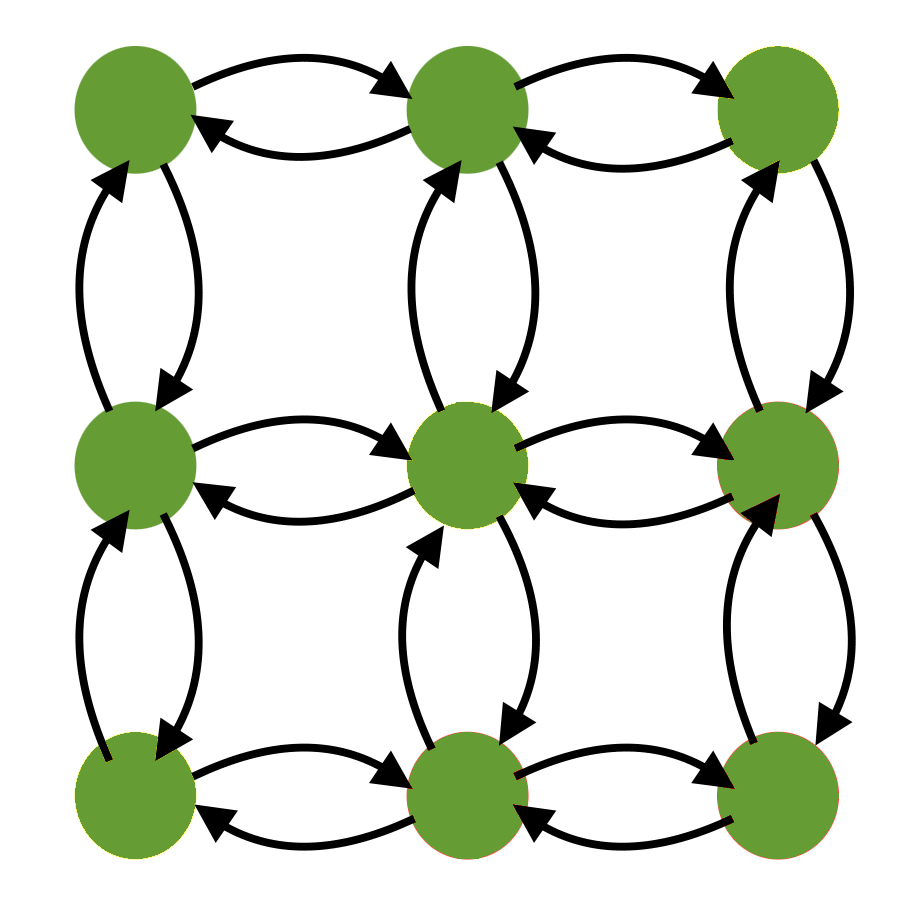
\includegraphics[width=0.9\textwidth]{images/od_populations.jpg}
          \end{minipage}\hfill
          \begin{minipage}[c]{0.67\textwidth}
            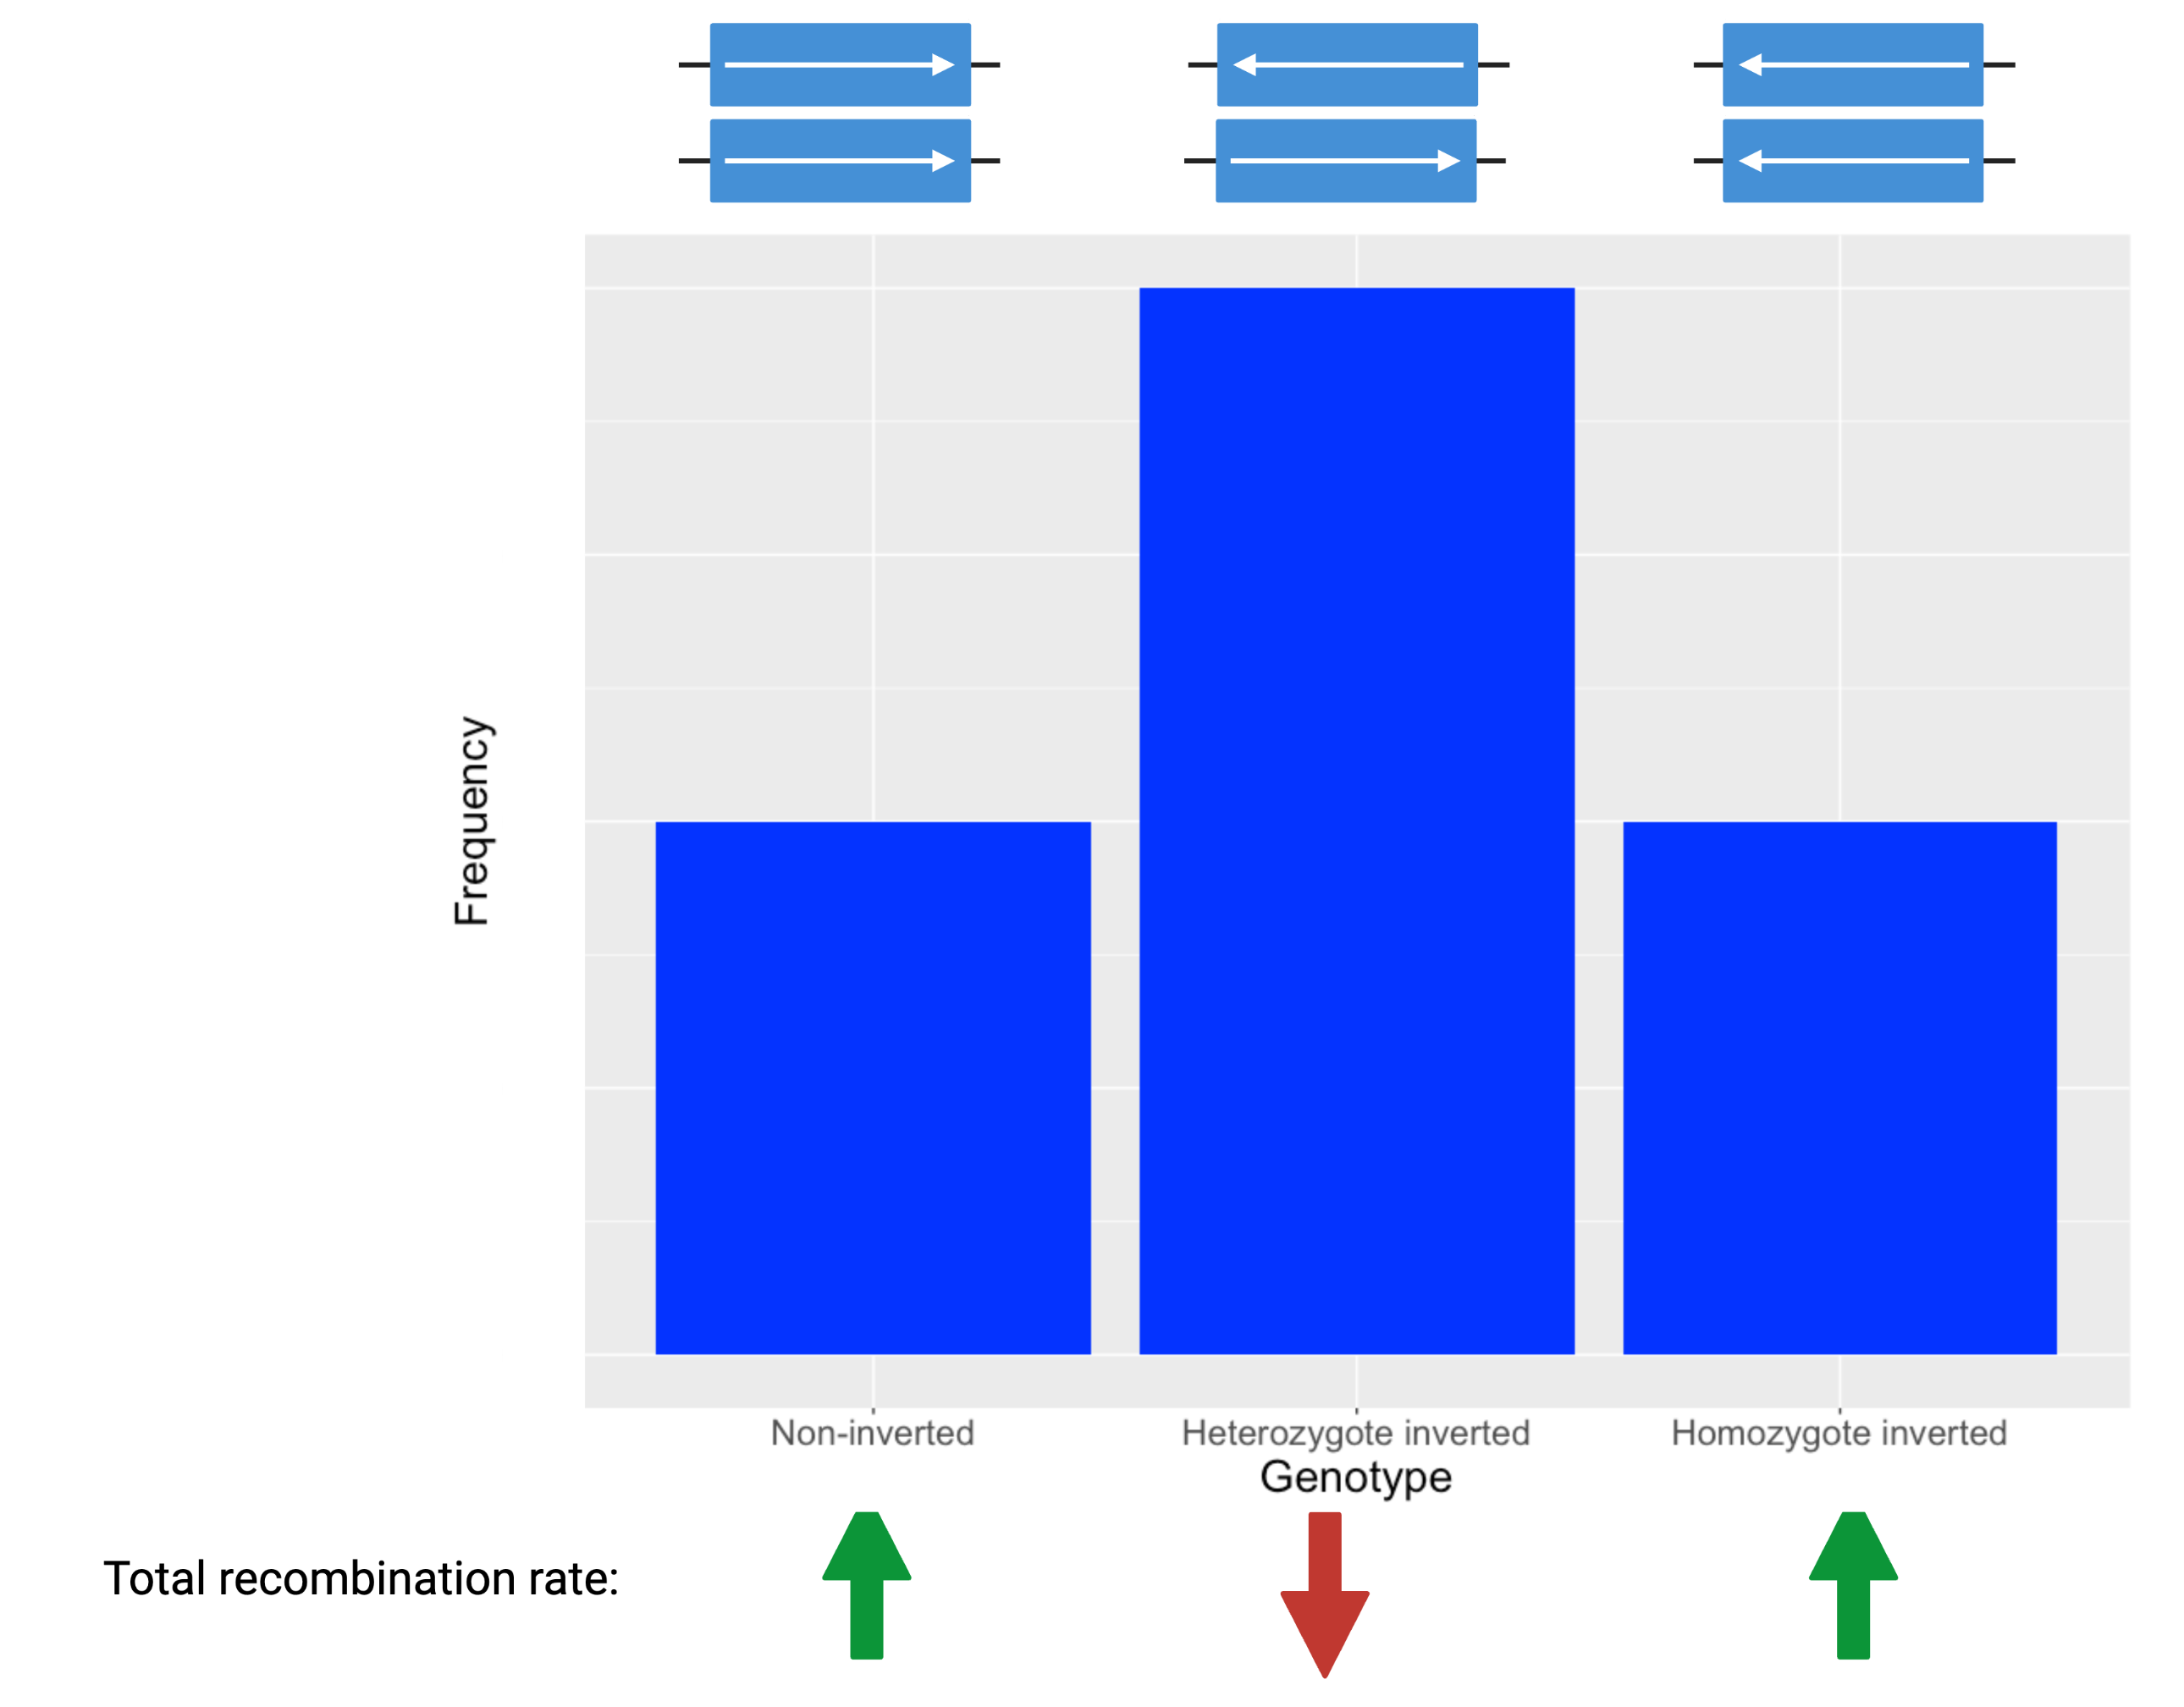
\includegraphics[width=0.9\textwidth]{figures/od_theory.png}
          \end{minipage}\hfill
          \caption{
            In the overdominant scenario, there were no population-dependent effects: all heterozygous individuals gained a fitness benefit. In this scenario, we would expect more heterozygotes over time, reducing the total recombination occurring in the population and increasing deleterious load.
            }
    \end{figure}

    In the overdominant scenario, individuals heterozygous for the inversion always gained a 10\% fitness benefit. Given the heterozygote advantage, we would expect more heterozygotes in the population over time. Since heterozygotes cannot undergo recombination, the total recombination occurring in the population is low. We expect this to result in deleterious build-up.

    \begin{figure}
    \centering
                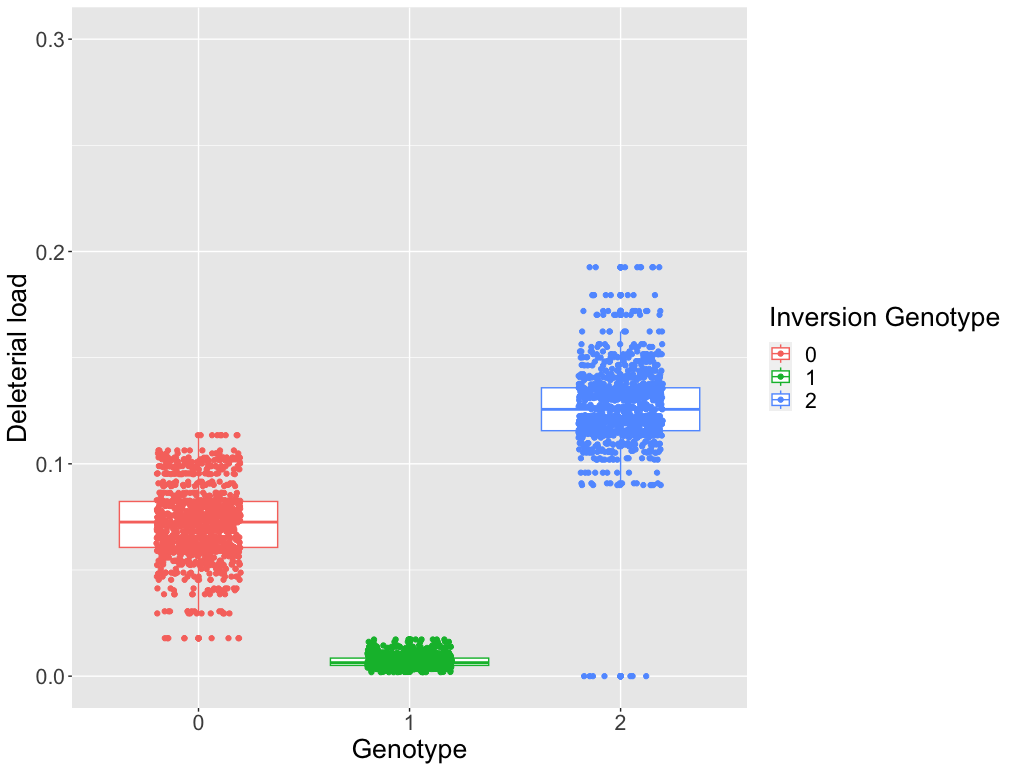
\includegraphics[width=0.5\textwidth]{figures/od_load_100kgen.png}
    \caption{An overdominant inversion scenario showed the least deleterious build-up in the heterozygote and the most in the homozygote.After the fitness modifier (+10\%) was removed, deleterious load was calculated as 1 - fitness. }
    \end{figure}

    \end{block}

    \begin{exampleblock}{Tentative overdominant results}

    In the overdominant scenario, non-inverted and \textbf{inverted homozygotes show greater deleterious load} than in the locally adaptive scenario. This shows that some increase in recombination is occurring, resulting in a \textbf{fitness rescue}. Unexpectedly, little deleterious build-up was observed in recombination-suppressed heterozygotes. Again, non-inverted individuals have a higher genetic load than expected, one reason for which could be genetic drift. Similar to the locally adaptive model, there are \textbf{unresolved questions}.



    \end{exampleblock}

  \begin{block}{References and Acknowledgements}

  \begin{figure}
    \begin{minipage}[c]{0.3\textwidth}
            
\includegraphics[width=0.5\textwidth]{images/qr.png}
          \end{minipage}\hfill
          \begin{minipage}[c]{0.67\textwidth}
              Special thanks to the other members in the Owens Lab and the University of Victoria Research Computing Services department.
          \end{minipage}\hfill
    \end{figure}

  \end{block}

\end{column}

\separatorcolumn
\end{columns}
\end{frame}

\end{document}
